\section{Gauge Freedom in the Landau Problem}
\label{sec:landau}

\subsection{The Landau Problem}

Next we investigated the degrees of gauge freedom present in the Landau problem
of a uniform everywhere magnetic field, $\mathbf{B} = B \basis{z}$. Of
particular interest is how the ground state wavefunction gains the freedom from
the choice of gauge. This is examined explicitly for the straight (sometimes
called the Landau) and for the circular (sometimes called symmetric) gauges,
with particular emphasis placed on the degeneracy of the circular gauge ground
state due to the $f(x,y)$ that appears in the wavefunction solution, that can be
any analytic function.

\subsection{The Straight Gauge}

In the straight gauge, $\mathbf{A} = Bx\basis{y}$, the ground state solution for
the wavefunction is
\begin{align}
    \Psi_{s,0}(x,t) = \mathcal{N} e^{- \frac{1}{2} \mymu x^2} e^{-i \frac{1}{2}
        \hbar \Omega t},
\end{align}
where $\mathcal{N}$ is a normalisation factor and $\Omega = \frac{qB}{m}$ is the
angular frequency of the solution \cite{murayama}. This ``Gaussian ridge''
wavefunction is plotted in Figure \ref{subfig:straight-wavefunction},
illustrating its invariance to translations in the $y$ direction.

The associated probability density and phase of the wavefunction are
\begin{align}
    \rho = \mathcal{N}^2 e^{- \mymu x^2} \\
    \mathrm{and}~ \theta = - \frac{1}{2} \hbar \Omega t,
\end{align}
and the probability current, as plotted in Figure \ref{subfig:straight-current},
is
\begin{align}
    \mathbf{J}_s &= \frac{\hbar}{m} \mathcal{N}^2 e^{- \mymu x^2} \left(
        \nabla \left\{ -\frac{1}{2} \hbar \Omega t \right\} - \frac{q}{\hbar} B
        x \basis{y} \right) \\
    &= - \Omega \mathcal{N}^2 e^{- \mymu x^2} x\basis{y} ~\mathrm{as}~
        \nabla \left\{ -\frac{1}{2} \hbar \Omega t \right\} = 0.
\end{align}

Importantly, this wavefunction is invariant under translations of both $y$ and
$z$, due to the choice of gauge. In a sense, the gauge freedom we have in
choosing $\mathbf{A}$ gives us the symmetry in $\Psi_{s,0}$.

\begin{figure}
    \centering
    \begin{subfigure}{0.45\linewidth}
        \centering
        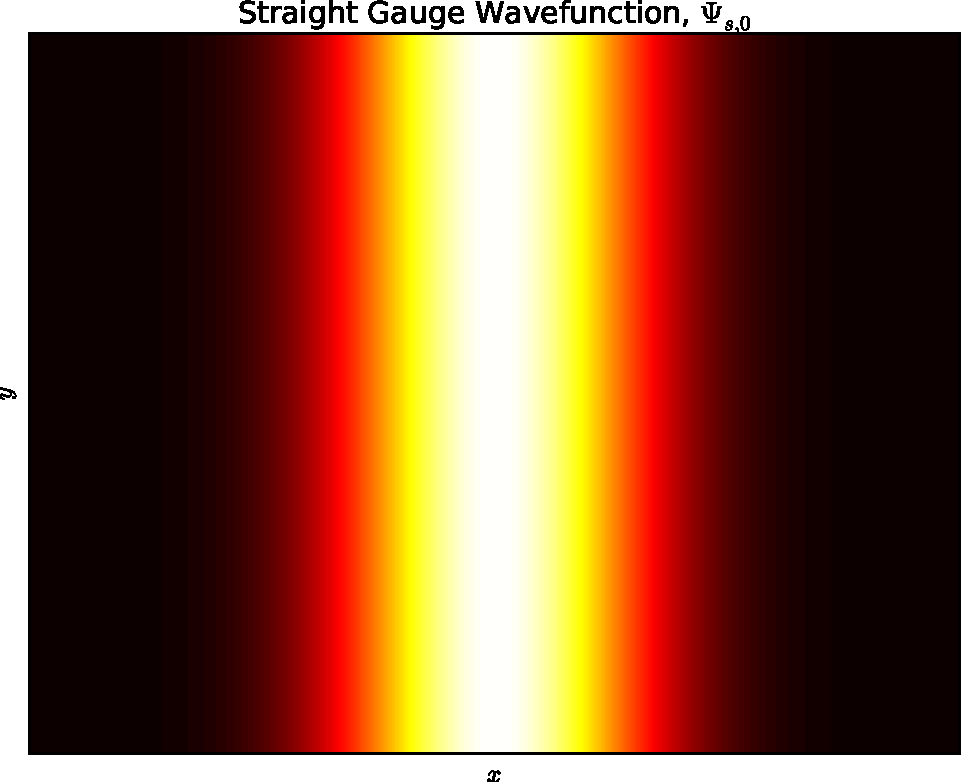
\includegraphics[width=\linewidth]{straight-gauge-wavefunction}
        \caption{The modulus of the ground state wavefunction. Note the
            independence of the $y$ coordinate.}
        \label{subfig:straight-wavefunction}
    \end{subfigure}
    \begin{subfigure}{0.45\linewidth}
        \centering
        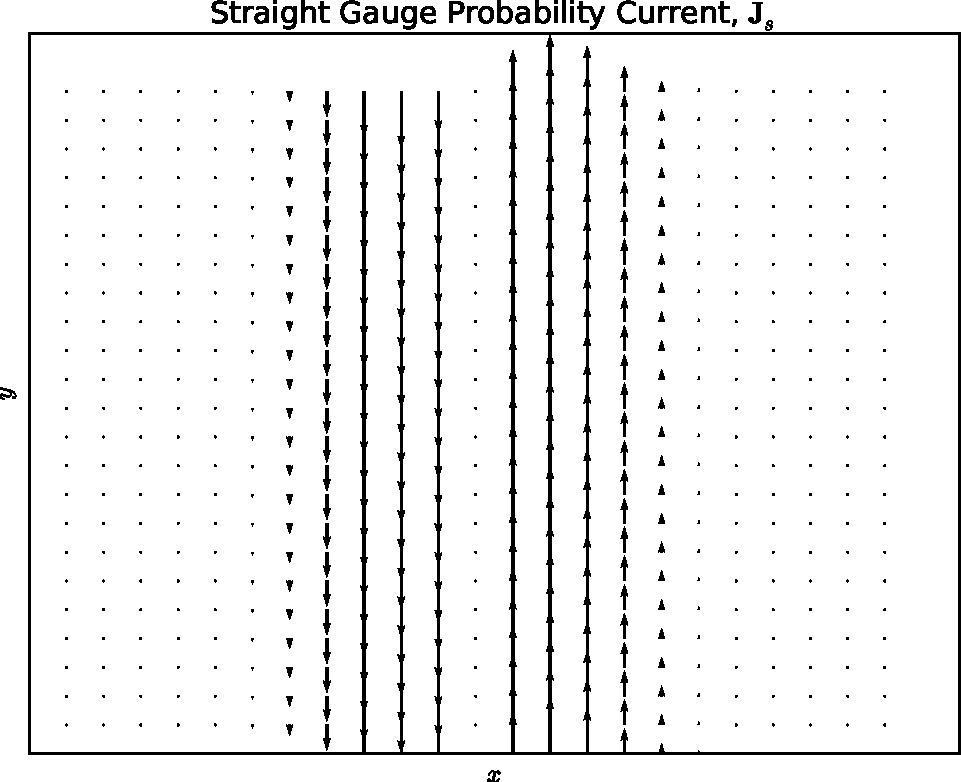
\includegraphics[width=\linewidth]{straight-gauge-current}
        \caption{The ground state probability current. Note that it points
            always in the $y$ or $-y$ directions.}
        \label{subfig:straight-current}
    \end{subfigure}
    \caption{Ground state and probability current solutions to the Landau
    problem in the straight gauge, $\mathbf{A} = Bx\basis{y}$.}
    \label{fig:straight}
\end{figure}

\subsection{The Circular Gauge}

When using the circular gauge, $\mathbf{A} = \frac{1}{2} B \left( x \basis{y} -
y \basis{x} \right)$, the ground state wavefunction is a two dimensional
``Gaussian bulge'':
\begin{align}
    \Psi_{c,0}(x, y, t) = \mathcal{N} f(x,y) e^{- \frac{1}{4} \mymu \left( x^2 +
        y^2 \right)} e^{-i \frac{1}{2} \hbar \Omega t},
\end{align}
where $f(x,y)$ is any complex analytic function \cite{murayama}. Figure
\ref{subfig:circular-wavefunction} shows that whereas before with the straight
gauge our wavefunction was invariant to translations in the $y$ directions, here
our wavefunction is invariant to rotations about the origin.

If we write the function $f(x,y)$ in terms of the modulus and phase as
$f(F,\phi) = Fe^{i \phi}$, then this wavefunction has probability density
\begin{align}
    \rho = \mathcal{N}^2 F^2 e^{- \frac{1}{2} \mymu \left( x^2 + y^2 \right)},
    \label{eqn:circular-density}
\end{align}
and the probability current corresponding to this wavefunction, as plotted in
Figure \ref{subfig:circular-current}, is
\begin{align}
    \mathbf{J}_c(f) = F^2 \mathcal{M} e^{- \mu
        \left( x^2 + y^2 \right)} \left( \nabla \phi - \mu \left(
        x\basis{y} - y\basis{x} \right) \right),
\end{align}
where $\mathcal{M} = \frac{\hbar}{m} \mathcal{N}^2$ and $\mu = \frac{1}{2}
\mymu$ for brevity.

\begin{figure}
    \centering
    \begin{subfigure}{0.45\linewidth}
        \centering
        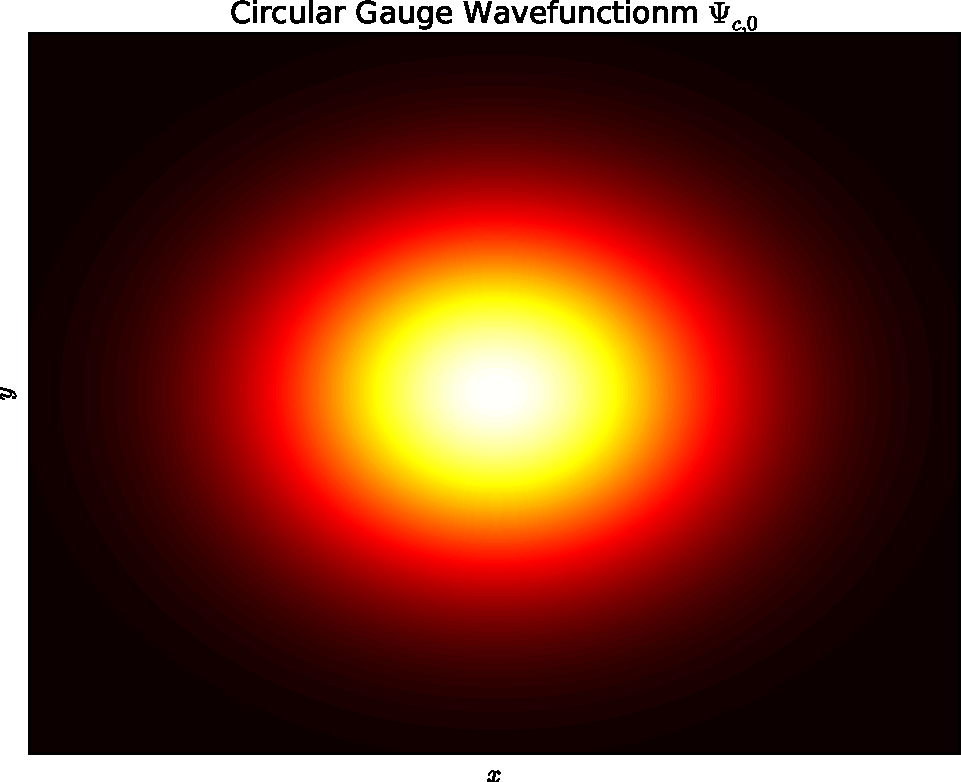
\includegraphics[width=\linewidth]{circular-gauge-wavefunction}
        \caption{The modulus of the ground state wavefunction solution to the
            Landau problem when using the circular gauge.}
        \label{subfig:circular-wavefunction}
    \end{subfigure}
    \begin{subfigure}{0.45\linewidth}
        \centering
        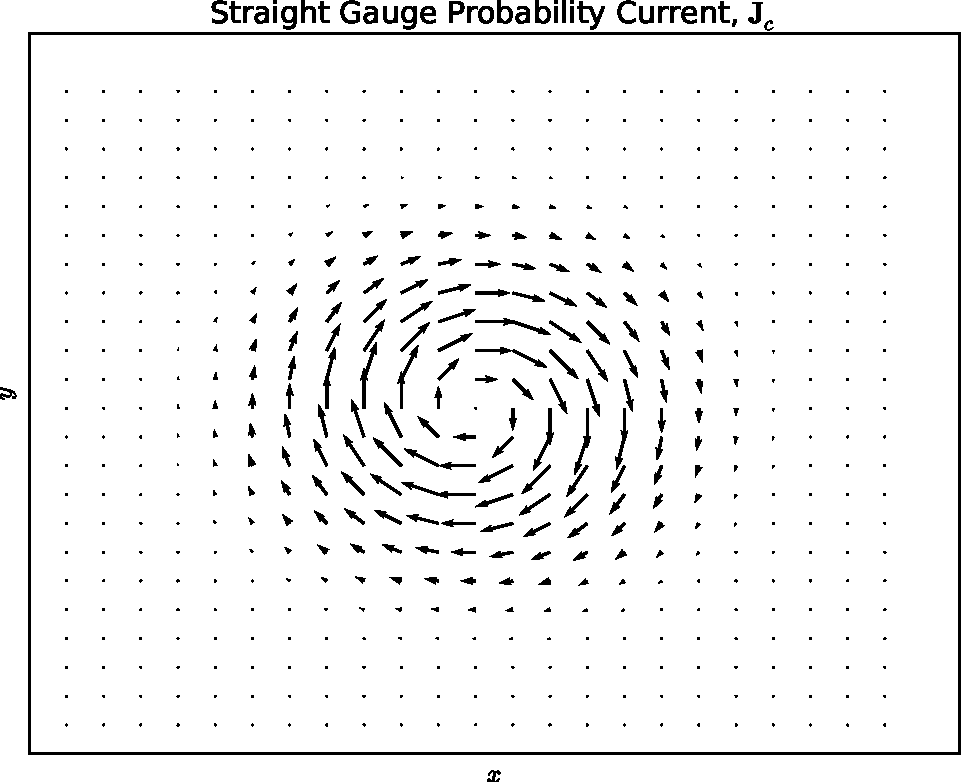
\includegraphics[width=\linewidth]{circular-gauge-current}
        \caption{The probability current corresponding to the ground state solution
            of the Landau problem, using the circular gauge.}
        \label{subfig:circular-current}
    \end{subfigure}
    \caption{The ground state wavefunction and probability current for the
        Landau problem using the circular gauge, $\mathbf{A} = \frac{1}{2} B
        \left( x\basis{y} - y\basis{x} \right)$.}
    \label{fig:circular}
\end{figure}

Whereas previously with the straight gauge the wavefunction is symmetric under
$y$ translations due to the choice of the gauge, now our wavefunction is
rotatinoally symmetric; choosing the gauge is equivalent to choosing the
symmetry of the resulting wavefunction.

Note how the probability current spins clockwise around the central peak of the
wavefunction. Additionally, the current points at all times parallel or
anti-parallel to the symmetry of the wavefunction; with the straight gauge there
is $y$ translation invariance due to our choice of gauge, and $\mathbf{J}_s$ points always in the $\pm y$
direction, while for the circular gauge there is rotational invariance due to
our choice of gauge, and
$\mathbf{J}_c$ always points tangentially. Note that the gauge is required to
have zero $z$ component, so this symmetry of the wavefunction is due to the
underlying magnetic field, \textit{not} the particular choice of gauge.

Of particular interest here is the analytic function $f(x,y)$, which gives an
infinite degeneracy to the ground state. This degeneracy is discussed further,
with reference to a comparison of the stringency of the continuity of the
resulting probability current.

\subsection{Equivalence of probability currents}

If we choose $f(x,y)$ to be
\begin{align}
    f_s(x,y) &= e^{- \frac{1}{4} \mymu \left( x + i y \right)^2} \\
             &= e^{- \frac{1}{4} \mymu \left( x^2 - y^2 \right)}
                e^{-i \frac{1}{2} \mymu xy},
\end{align}
(which being a function of just $z$ and not $z^*$ is analytic), then the modulus
and phase of the wavefunction are
\begin{align}
    F_s &= e^{- \frac{1}{4} \mymu \left( x^2 - y^2 \right)} \\
    \mathrm{and}~ \phi_s &= -\frac{1}{2} \mymu xy.
\end{align}
Thus, the probability current is
\begin{align}
    \mathbf{J}_c(f_s)
    &= F_s^2 \mathcal{M} e^{- \mu \left( x^2 + y^2 \right)}
       \left( \nabla \phi_s - \mu \left( x\basis{y} -
       y\basis{x} \right) \right) \\
    &= e^{- \mu \left( x^2 - y^2 \right)} \mathcal{M} e^{- \mu \left( x^2 + y^2
       \right)} \left( \nabla \left\{ - \mu xy \right\} - \mu \left( x\basis{y} - y
       \basis{x} \right) \right) \\
    &= - \mathcal{M} \mu e^{- \frac{1}{2} \frac{M
       \Omega}{\hbar} x^2} \left( \nabla \left\{ xy \right\} + x\basis{y} -
       y\basis{x} \right) \\
    &= - \mathcal{M} \mu e^{- \frac{1}{2} \frac{M
       \Omega}{\hbar} x^2} \left( x\basis{y} + y\basis{x} + x\basis{y} -
       y\basis{x} \right) \\
    &= - \Omega \mathcal{N}^2  e^{- \frac{1}{2} \frac{M \Omega}{\hbar} x^2}
       x\basis{y} \\
       &= \mathbf{J}_s.
\end{align}

What this means is that one can choose a particular value of $f(x,y)$ for which
the circular gauge reduces to the straight gauge. This raises the interesting
question of whether all values of $f(x,y)$ are permitted, and whether the
$\mathbf{J}_c(f)$ currents form a basis for all the possible $\mathbf{J}$
values.

\subsection{Locking the analyticity of $f(x,y)$ to continuity}

Here we demonstrate that all functions of $f(x,y)$, provided they are analytic
with no other constraints, produce a respectable or physical probability
current. In other words, the associated probability current $\mathbf{J}_c(f)$
satisfies the continuity equation (Equation \ref{eqn:continuity}). Here
$\Psi_{c,0}(x, y, t)$ has $\rho = \mathcal{N}^2 F^2 e^{- \frac{1}{2} \mymu
\left( x^2 + y^2 \right)}$ as per Equation \ref{eqn:circular-density}. Thus
\begin{align}
    \dot \rho &= \frac{\partial}{\partial t} \left( \mathcal{N}^2 F^2 e^{-
        \frac{1}{2} \mymu \left( x^2 + y^2 \right)} \right) \\
    &= 0,
\end{align}
and the continuity equation is simply
\begin{align}
    \nabla \cdot \mathbf{J}(f) = 0.
\end{align}
So showing that all values of $f(x,y)$ produce respectable probability currents
means showing that
\begin{align}
    \nabla \cdot \mathbf{J}_c(f) = 0, ~\forall f=f(x,y).
\end{align}
To demonstrate this, we first make two observations of the consequences of the
analyticity of $f(x,y)$.

\subsubsection{Analyticity of $f(x,y)$}

If we call the real and imaginary components of $f(x,y)$
\begin{align}
    f_R = \Ree{f(x,y)} ~\mathrm{and}~ f_I = \Imm{f(x,y)},
\end{align}
then these real and imaginary components are both harmonic, i.e. they obey
Laplace's equation:
\begin{align}
    \nabla^2 f_R &= \partial_x^2 f_R + \partial_y^2 f_R = 0 \\
    \mathrm{and}~ \nabla^2 f_I &= \partial_x^2 f_I + \partial_y^2 f_I = 0 \\
    \Rightarrow \nabla^2 f(x,y) &= \nabla^2 f_R + \nabla^2 f_I = 0.
\end{align}
Additionally, $f_R$ and $f_I$ obey the Cauchy-Riemann equations:
\begin{align}
    \partial_x f_R &= \partial_y f_I \\
    \mathrm{and}~ \partial_y f_R &= - \partial_x f_I
\end{align}

\subsubsection{Analyticity of $\logg{f(x,y)}$}

For any function $g(z)$, if $g(z)$ is analytic on $\mathbb{C}$, then the
principal branch of $\logg{g(z)}$ is analytic on $\mathbb{C} \setminus \left\{
g(z) \in \mathbb{R} : g(z) \le 0 \right\}$.
% TODO: Find reference confirming this (no, not Math Overflow).

Thus, if we take the principal branch of $\log$, and discard the negative real
line $f(x,y) \in \mathbb{R}:f(x,y) \le 0$, then $\logg{f(x,y)}$ is also
analytic, and the real and imaginary parts of this are also harmonic;
\begin{align}
    \logg{f(x,y)} &= \logg{F} + i \phi \\
    \Rightarrow \Ree{\logg{f(x,y)}} &= \logg{F} \\
    \mathrm{and}~ \Imm{\logg{f(x,y)}} &= \phi
\end{align}
are the real and imaginary components, so the harmonicity implies that
\begin{align}
    \nabla^2 \Ree{\logg{f(x,y)}} &= \nabla^2 \logg{F} = 0 \\
    \mathrm{and}~ \nabla^2 \Imm{\logg{f(x,y)}} &= \nabla^2 \phi = 0.
\end{align}

In addition, $\logg{F}$ and $\phi$ also obey the Cauchy Riemann equations;
\begin{align}
    \partial_x \logg{F} &= \partial_y \phi
    \label{eqn:log-cr-1} \\
    \mathrm{and}~ \partial_y \logg{F} &= - \partial_x \phi
    \label{eqn:log-cr-2}
\end{align}

A consequence of this is that $\nabla F \cdot \nabla \phi = 0$. This can be
shown simply in components as
\begin{align}
    \nabla F \cdot \nabla \phi
        &= \colvec{\partial_x F}{\partial_y F}{0} \cdot
        \colvec{\partial_x \phi}{\partial_y \phi}{0} \\
        &= \colvec{\partial_x F}{\partial_y F}{0} \cdot
        \colvec{- \partial_y \logg{F}}{\partial_x \logg{F}}{0} \\
        &= \frac{1}{F} \colvec{\partial_x F}{\partial_y F}{0} \cdot
        \colvec{- \partial_y F}{\partial_x F}{0} ~\mathrm{as}~ \partial_u
        \logg{F} = \frac{\partial_u F}{F}, ~\forall u \\
        &= 0
\end{align}

Using these facts, the divergence of $\mathbf{J}_c$ can be expressed as
\begin{align}
    \div{J}_c - -2\mu F^2 \mathcal{M} e^{-\mu\left(x^2 + y^2\right)} \left[
        \nabla \logg{F} \cdot \left( x\basis{y} - y\basis{x} \right) + \nabla
        \phi \cdot \left( \mathbf{x} + \mathbf{y} \right) \right]
    \label{eqn:div-j}
\end{align}

\Cref{eqn:log-cr-1,eqn:log-cr-2} allow us to express $\nabla \phi$ as
\begin{align}
    \nabla \phi = \basis{z} \times \nabla \logg{F},
\end{align}
which means that by the cyclic permutation of the scalar product
\begin{align}
    \nabla \phi \cdot \left( \mathbf{x} + \mathbf{y} \right)
    &= \left( \basis{z} \times \nabla \logg{F} \right) \cdot \left( \mathbf{x} +
        \mathbf{y} \right) \\
    &= \nabla \logg{F} \cdot \left[ \left( \mathbf{x} + \mathbf{y} \right)
        \times \basis{z} \right] \\
    &= - \nabla \logg{F} \cdot \left( x\basis{y} - y\basis{x} \right).
\end{align}

Thus, the bracketed term in \Cref{eqn:div-j} cancels and the divergence of
$\mathbf{J}_c$ is zero for all analytic functions $f(x,y)$.

\subsection{Strictness of $\mathbf{J}$ versus $f(x,y)$}

So we have established that for every $f(x,y)$ there corresponds a
divergenceless $\mathbf{J}$, so the natural question to ask next is whether any
given $\mathbf{J}$ has a corresponding analytic function $f(x,y)$.

In other words, is the condition of analyticity of $f(x,y)$ stronger than the
condition of divergencelessness of $\mathbf{J}$, or are they equally as
stringent conditions. Logically this could be expressed as
\begin{align}
    f(x,y) ~\mathrm{is~analytic}~ &\implies \div{J} = 0 \\
    \mathrm{versus}~ f(x,y) ~\mathrm{is~analytic}~ &\iff \div{J} = 0.
\end{align}

Being a complex function, $f(x,y)$ is essentially two function of two variables,
$f_R(x,y)$ and $f_I(x,y)$; the constraint of analyticity simply says that the
real and imaginary parts of this function of two variables are related by the
Cauchy-Riemann equations.

The condition of analyticity on a complex function is extremely stringent;
unlike in real analysis, complex analyticity implies infinite differentiability.
% TODO: Find a reference for this, or is it not entirely relevant
An important result of complex analysis is that any analytic real function can
be extended or analytically continued into an analytic function on the entire
complex plane. This means that any complex function can be uniquely specified by
its value on the real axis. Thus, any analytic function $f(x,y)$ is entirely
determined by the value along the real axis, $f(x,0)$. Thus, $f(x,y)$ is
essentially two functions $f_R$ and $f_I$ of one variable, $x$. These two
functions aren't independent, however, due to Cauchy-Riemann.

The condition of divergencelessness on the probability current means that $J_x =
- J_y$. Thus $\mathbf{J}$ is essentially one function of two variables, $x$ and
$y$. In this plane, this single function representing the divergenceless
probability current can have any value; it is unrestrained.

A divergenceless quantity can therefore still take unique values across the
whole $x,y$ plane, whereas an analytic function is entirely uniquely determined
by just the $y = 0$ line. Therefore, the condition of analyticity is more
stringent than the condition of continuity; every analytic $f(x,y)$ has a
corresponding divergenceless $\mathbf{J}_c$, but not every divergenceless
$\mathbf{J}$ has a corresponding $f(x,y)$.
